%%%%%%%%%%%%%%%%%%%%% chapter.tex %%%%%%%%%%%%%%%%%%%%%%%%%%%%%%%%%
%
% sample chapter
%
% Use this file as a template for your own input.
%
%%%%%%%%%%%%%%%%%%%%%%%% Springer-Verlag %%%%%%%%%%%%%%%%%%%%%%%%%%
%\motto{Use the template \emph{chapter.tex} to style the various elements of your chapter content.}
\chapter{Acoustic Principals}
\label{Introduction}
Acoustics is a branch of physics\footnote{though often considered to be interdisciplinary} that aims to characterise behaviours of Newton's second law of motion applied to mechanical wave propagation and obeying the physical conservation law~\cite{beranek1954acoustics}. This characterisation of sound propagation is intrinsically linked to many other disciplines of science and engineering, as well as psychological and perceptual study. In this section we will review the acoustic wave equation, and discuss some acoustic equations of interest in large room electroacoustics.

\section{The Acoustic Wave Equation}

Acoustic waves are classified as fluctuations of pressure in a given medium, manifesting as longitudinal waves of high and low pressure and air density~\cite{Rossing2007}. These fluctuations are often cyclical in nature around an ambient pressure that is some times assumed to be 1 atmospheric pressure at sea level or $101.35kPa$. Similar to the behaviour of heat convection or fluid diffusion, these cyclical fluctuations propagate and spread through the medium of interest, decaying towards a resting steady state. It is possible to calculate an approximate solution to the propagation of pressure through a space, by solving a system of second order partial differential equations that can be collected into a 'Wave Equation'. Below, we will introduce the three building blocks of the wave equation in one dimensional space. These building blocks are Newton's Second Law of Motion, the gas law, and the laws of conservation of mass.\\

In the Mcgraw-Hill Electronic and Electrical Engineering Series of books, the late Leo Beranek authored the Acoustics volume~\cite{beranek1954acoustics}. This reference text contains an elegant summary of the wave equation in 1 dimension in standard notation, and 3 dimensions in vector notation. Rienstra published an introduction to acoustics text~\cite{Rienstra1952} that takes a strong stance from a fluid dynamics perspective, and is well worth reviewing for a more in-depth derivation than is presented in this text. To consider the wave equation, we should use the analogy of a small volume of gas, within a significantly larger homogeneous medium. The faces of the volume are frictionless, and only the pressure at any face impacts on the gas inside the volume.\\

\subsection{Wave Equation In One Dimension}
\subsubsection{Equation Of Motion}

Sound pressure $p$ propagates across the larger medium like a plane wave, from one side to the other in the $x$ direction at a rate equal to the change in space: $\frac{\delta p}{\delta x}$\\
Force acting on the volume in the positive $x$ direction can thus be described as:
\begin{center}
 $-(\frac{\delta p}{\delta x} \Delta x) \Delta y \Delta z$\\
\end{center}
Assuming that the balance of force across the volume over a slice of time is equal to the unit size of the volume and the speed of the wave.\\
A positive gradient causes acceleration in the $-x$ direction, and a negative gradient causes acceleration of the volume in the $+x$ direction.\\
Force $\textit{f}$ per unit volume $V$ is given by dividing both sides of the previous equation by the area of the volume:
\begin{center}
 $V = \Delta x \Delta y \Delta z$, $\frac{\textit{f}}{V} = -\frac{\delta p}{\delta x}$\\
\end{center}
Newton's second law of motion dictates that the rate of change of momentum in the volume must balance with force per unit volume, and we assume the mass $M$ of gas in the volume is constant. The force mass balance can be described as:
\begin{center}
 $\frac{\textit{f}}{V} = -\frac{\delta p}{\delta x} = \frac{M}{V} \frac{\delta u}{\delta t} = \rho^{\prime}\frac{\delta u}{\delta t}$\\ 
\end{center}
Where $u$ is the velocity of gas in the volume, $\rho^{\prime}$ is the density of the gas, and $M = \rho^{\prime} V$ is the mass of gas in the volume.\\
If the change in density of gas in the volume is sufficiently small, the $\rho^{\prime}$ will be approximately equal to the average density $\rho_0$, thus simplifying the equations above to:
\begin{center}
 $-\frac{\delta p}{\delta x} = \rho_0 \frac{\delta u}{\delta t}$\\
\end{center}
Which is the momentum equation.\\
\subsubsection{Gas Law}
This approximation may be appropriate as long as the absolute maximum pressure is relatively low, so that the behaviour of the air may be assumed to be linear and other assumption can be made that will be discussed shortly.\\
Assuming that the gas in the volume is ideal, the gas law $ PV = RT $ should hold true. Here, T is the temperature in degrees Kelvin, and R is a constant based on the mass of the gas. For this approximation we assume that the system is adiabatic and that compression an expansion are sufficiently fast to make the thermal effects negligible, and that T and R are lumped into a gas constant which for air is $\gamma \approx 1.4$.\\

In differential form the relationship between pressure and volume for an adiabatic expansion of the volume is $\frac{\delta P}{P} = \frac{-\gamma  \delta V}{V} $ i.e. changes in pressure scale with changes in volume by this $\gamma$ value.\\

If perturbations in pressure and volume due to a sound wave ($p$ for pressure and $\tau$ for volume respectively) are sufficiently small compared to the rest values $P_0$ and $V_0$, the time based derivative of the above equation can be written as follows: 
\begin{center}
$\frac{1}{P_0} \frac{\delta p}{\delta t} = \frac{-\gamma}{V_0} \frac{\delta \tau}{\delta t}$\\
\end{center}
This equation shows the balance between the proportional changes in pressure and volume over time, with a scaling of the change of the volume by the constant $\gamma$. \\
\subsubsection{Conservation Of Mass}
As this wave equation is concerned with the transport of pressure within a volume and not just the aggregate pressure of the volume with respect to the surrounding medium, a continuity expression must be applied. The conservation of mass states that the total mass of gas in the volume must remain constant. This conservation law brings a unique relationship between discrete velocities at the boundary of the volume. If the volume is displaced by some rate $\epsilon_x$, air particles at either boundary of the volume at some point in time must be displaced at an equal rate for the mass of the volume to remain constant. As such if the left side of the volume is displaced with a velocity, in a given time the particles at the right hand boundary must also be displaced. This general displacement term can be written as:
\begin{center}
 $\epsilon_x + \frac{\delta \epsilon_x}{\delta x} \Delta x$\\
\end{center}

The change of velocity with respect to the volumes dimension gives:
\begin{center}
$\tau = V_0\frac{\delta \epsilon_x}{\delta x} \Delta x$.\\
\end{center}

Differentiating this with respect to time gives:
\begin{center}
 $\frac{\delta \tau}{\delta t} = V_0\frac{\delta u}{\delta x}$\\
\end{center}
Where $u$ is the instantaneous particle velocity.\\
\subsubsection{Wave Equation}
The one dimensional wave equation can be created by combining the above statements about Newtons second law of motion, the gas law and the continuity equation. The combination of the gas law and continuity equation gives:
\begin{center}
$\frac{\delta p}{\delta t} = -\gamma P_0\frac{\delta u}{\delta x}$.\\
\end{center} 

Which differentiated with respect to time gives:
\begin{center}
$\frac{\delta^2 p}{\delta t^2} = -\gamma P_0\frac{\delta^2 u}{\delta t \delta x}$.\\
\end{center} 

Differentiating the momentum equation derived above with respect to time gives:
\begin{center}
 $-\frac{\delta^2 p}{\delta t^2}=\rho_0\frac{\delta^2 u}{\delta x \delta t}$\\
\end{center}

Combining the above equations gives the equation for pressure transport with respect to time:
\begin{center}
 $\frac{\delta^2 p}{\delta x^2}=\frac{\rho_0}{\gamma P_0}\frac{\delta^2 p}{\delta t^2} $\\
\end{center}

If c is defined as the speed of propagation in the medium of interest:
\begin{center}
$c^2\approx \frac{\gamma P_0}{\rho_0}$\\
\end{center} 
This is true~\cite{beranek1954acoustics} when making the assumption that:
\begin{center}
$c \approx (1.4\frac{10^5}{1.2})^\frac{1}{2}$\\
\end{center}
Where:
\begin{itemize}
\item ambient air pressure at sea level is $10^5Pa$
\item  1.4 is the adiabatic constant $\gamma$ (ratio of specific heats) for air
\item the density of air $\rho_0 \approx 1.2kg/m^3 $
\end{itemize}

The 1 dimensional wave equation is defined in terms of pressure fluctuation over space for time as:
\begin{center}
 $\frac{\delta^2 p}{\delta x^2}=\frac{1}{c^2}\frac{\delta^2 p}{\delta t^2}$\\
\end{center}
This equation can also be expressed in terms of the instantaneous velocity in the volume over time as:
\begin{center}
 $\frac{\delta^2 u}{\delta x^2}=\frac{1}{c^2}\frac{\delta^2 u}{\delta t^2}$\\
\end{center}

In the above section the wave equation has been derived with forms of velocity and pressure as the independent variables. We have also shown that pressure, velocity, displacement and density are related within the system of equations, by differentiating and integrating with respect to space and time. As these forms of the wave equation are intrinsically coupled, it is possible to leverage this coupling when generating a numerical solution to the wave equation. It is also important to note that a significant number of assumptions have been made when deriving these equations, and any solution to these equations may only be accurate when simulating a loss free, frictionless, homogeneous, ideal gas medium, where all perturbations are sufficiently small and fast that it is possible to reduce the complexity of the system.\\

\section{Acoustic Properties of Interest in This Study}
Having derived a wave equation to simulation acoustic propagation, it is important to have an understanding of what acoustic phenomena can be observed through solving the wave equation. This study is interested in solving large domains efficiently, and next section will discuss three components of acoustics behaviour that may relate to large room acoustics.\\

\subsection{Inverse Square Law \& Propagation time}
As previously noted, sound propagates as longitudinal waves through a medium such as air or water. These waves are often conceptualised as simple rays~\cite{beranek1954acoustics} travelling through a space\footnote{It may be appropriate to often consider space to be 3 dimensional (3D), or a lower order approximation of a 3D space}, much like planar waves. However, the properties of a sound source such as the directivity and shape can have a significant effect on the behaviour of sound wave propagation. An example of this is the difference in energy spread over distance for theoretically ideal point and line sources. Ideal point sources that propagate sound omni-directionally obey the inverse square law and propagate sound spherically, and ideal line sources do not as they propagate sound cylindrically. The inverse square law is sound propagations is defined as~\cite{Davis2014}\\
\begin{center}
$I = \frac{P}{4 \pi r^2}$\\
\end{center}
Where I is the intensity over the area of the sphere, P is the propagated energy at the source and r is the radius of the sphere i.e. the distance between the source and the point of inquiry. This equation denotes that as an acoustic pressure wave radiates outward like an expanding sphere, as the area of the surface of the sphere increase the energy-per-unit-area of the surface of the sphere decreases. That is, as $r$ increases, $ I $ decreases, assuming $ P $ is a constant pressure of interest.\\
As ideal line sources propagate pressure waves cylindrically, the equation above can be modified to account for this change:\\
\begin{center}
$I = \frac{P}{2 \pi r}$\\
\end{center}
These two similar equations show a change in relationship between acoustic power over distance for different acoustic sources. If you were to evaluate the change of $I$ for different values of $r$ with the point source equation, you would find that as $r$ is doubled $I$ decreases by $6dB$. Doing the same for the line source equation would yield a $3dB$ change. This is in part due to the fact that we assume the cylinder is infinitely long, and thus we are evaluating a 2D simplification of a 3D problem. The area of the cylinder for any value of $r$ is less than the equivalent sphere, and so the theoretical distribution of energy is also reduced. This may be an important concept when considering the 2D approximation of 3D simulations in acoustic studies. Below is a graph showing the difference between intensity over distance for an ideal point and line source:\\

Although the wave equation considered and solved in this study is lossless i.e. we do not consider viscous or thermal losses in the basic linearised acoustic wave equation, we would expect to see a reduction in absolute pressure between a source and receiver. As sound travels at some finite distance over time $c$, we would also expect to see a uniform time between a wave being radiated from a source, and being recorded at some receiver location for all simulation methods\footnote{For an interesting review of the relationship between 1D, 2D and 3D sound propagation being derivative, please see the appendices}.\\ 

\subsection{Reverberation}
For this study we will consider spaces or domains of finite size. These domains have boundaries, and those boundaries will absorb and reflect sound waves by some proportion. In acoustic engineering the proportion of sound energy absorbed or reflected by a material is often described as an absorption or reflection coefficient $\alpha$, which is often expressed as a normalised value between 0 (totally reflecting) and 1 (totally absorbing)~\cite{beranek1954acoustics}. When considering boundaries to have frequency dependent absorption characteristics, a series of absorption coefficients are often attributed to frequency bands and these coefficients are usually real and not complex numbers.\\

If a sound source propagates a signal of appropriate amplitude, the sound wave will reach the boundaries and be partially absorbed or reflected in reciprocal directions. These reflections will continue to reflect and scatter, and will eventually decay beyond audibility. The reverberant sound field is the steady-state of diffusely scattered sound energy (reflections), due to perturbation by a sound source in bounded space. The amplitude of the sound source and diffusely scattered reflections balance with the rate of decay (diffusion and absorption) of the sound field~\cite{Everest2009}. In this case, the sound field can be conceptually split proportionally into direct and reverberant fields.\\

\subsubsection{Acoustic Absorption}
The decay rate of a reverberant sound field is often quantified by the time taken for a steady state sound field to reduce in level by $60{dB}$, once the sound source has finished propagating. This is defined as the $RT_{60}$ of the domain, and was first proposed by WC Sabine in 1900~\cite{Everest2009}. There have been a multitude of expansions on Sabines original formula, notably the Norris-Eyring~\cite{Beranek2006} equation which expanded the denominator of the reverberation time equation to allow for more realistically distributed absorption values above $0.1$. The Norris-Eyring reverberation time equation is as follows~\cite{Davis2014}:\\
\begin{center}
$T = 0.161\frac{V}{-S \ln(1 - \alpha)} $\\
Where $S$ is the surface area, $V$ is the volume of the domain and $\alpha$ is the average absorption coefficient and can be calculated as such:\\
$\alpha = (\left( S_{leftwall} \alpha_{leftwall})+(S_{rightwall} \alpha_{rightwall})+... \right) /S_{total}$ \\
\end{center}
The use of $RT_{60}$ as the preferred metric of decay time is valid, assuming that the acoustics system is linear and time-invariant.
A more comprehensive description of reverberation and overview of the associated parameters is given by Rossing~\cite{rossing2007springer}. \\

Low order reflections often described as early reflections in relation to psychoacoustics, may occur above the steady state amplitude (echos)~\cite{Everest2009} if the steady state amplitude decreases appropriately. Early and strong reflections are of significant interest in acoustic modelling, and the auralization and perception of sound fields due to the cues humans receive from perception of them e.g. room size and source direction information.\\

\subsubsection{Modified Hopkins-Stryker Equation}
The Modified Hopkins-Stryker equation presented by Beranek and modified by Peutz and Davis~\cite{Davis2014} can be used to approximate the level of sound at a point in a domain due to the direct and reverberant sound field:\\
\begin{center}
$L_T = L_W + 10 \log \left( \frac{Q M_e}{4 \pi D_x^2} + \frac{4 N}{S_\alpha M_a} \right) + K$
\end{center}
Where:
\begin{itemize}
\item $L_T =$ Total Level in $dB$
\item $L_W =$ Source Level at $D_x$ in $dB$
\item $D_x =$ Distance To Receiver 
\item $M_e =$ Direct Sound Modified i.e. Receiver Directivity
\item $Q =$ Directivity Factor of Source at $D_x$
\item $N =$ Radiated Acoustic Power
\item $M_a =$ Architectural Modifier to accommodate non-ideal absorption distribution
\item $S_\alpha =$ Total Absorption in Sabines
\item $K =$ Unit scaler i.e. 10.5 for SI unit measurements such as meters
\end{itemize}
In large domains as $D_x$ gets sufficiently far, $L_W$ and $N$ have to increase to meet the same levels as in a smaller space. Multiple loudspeakers with a high $Q$ are often implemented   to cover larger domains and further distances, thus increasing the value of $N$ and dominating the reverberant term in the equation. As long as the $M_a$ term is sufficiently small and the $S_\alpha M_a$ term is sufficiently high, the direct sound will dominate. However, in many large spaces such as arenas and stadiums, the $S$ term will be very large and the $\alpha$ will often be significantly small, thus causing reverberation to be a problem in sound re-enforcement where the loudspeaker system is not powerful enough. The Modified Hopkins-Stryker equation relies  on the same assumptions and ideal behaviour such as reverberation begin a stochastic process and the domain being ergodic i.e. absorption being evenly distributed, and so may not be an ideally accurate way to predict the behaviour. 

\subsection{Room Modes}
As the domains of interest in this study are fully bounded (much like a room), sound waves propagating in the domain are subject to periodicity relative to the dimensions of the domain. That is at wavelengths relative to the dimensions of the domain, standing waves may occur within the domain i.e. there will be regions maximal and minimal pressure change at points $\frac{\lambda}{4}$ relative to a dimension of the domain, where $\lambda$ is the spatial dimension of one cycle otherwise known as a wavelength. These standing waves are often called room modes, and for oblique modes in a 3 dimensional rectangular domain the frequencies of the  modes can be calculated as such:\\
\begin{center}
$\textit{f}_{n_xn_yn_z} = \frac{c}{2} \sqrt{\left(\frac{n_x}{l_x}\right)^2 + \left(\frac{n_y}{l_y}\right)^2 + \left(\frac{n_z}{l_z}\right)^2} $\\
Where $n_x, n_y, n_z$ is the order of the standing wave in the dimension.\\
\end{center} 

These modes are defined in spatial reciprocity as axial, tangential and oblique, depending on the order of dimensions involved in the periodicity i.e. When using such an equation as that above to calculate the theoretical modes of a rectangular domain, a state table such as the one below may be used to define the $n_{x/y/z}$ order \footnote{number of cycles within the dimension} component of each term:\\

\begin{center}
\begin{tabular}{|c|c|c|c|} 
  \hline
 Mode Type & x order & y order & z order \\
 \hline
 Axial & 0 & 0 & 1 \\ 
 Axial & 0 & 1 & 0 \\  
 Axial & 1 & 0 & 0 \\
 Tangential & 0 & 1 & 1 \\ 
 Tangential & 1 & 1 & 0 \\  
 Tangential & 1 & 0 & 1 \\
 Oblique & 1 & 1 & 1 \\ 
 Oblique & 1 & 1 & 2 \\  
 Oblique & 1 & 2 & 1 \\        
 \hline
\end{tabular}\\
\end{center}

In a room of the dimensions $5m$ by $4m$ by $3m$, modes up to the 10th order may occur at the following frequencies:\\

\begin{figure}[H]
\centering
  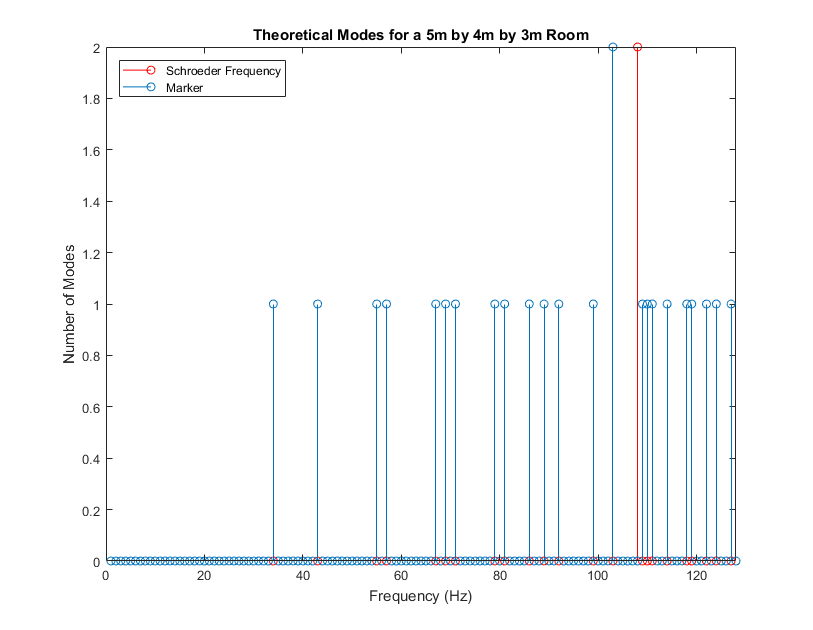
\includegraphics[width=\textwidth]{./graphics/modesuptoschr.png}
  \caption{Room Modes up to Schroeder Frequency for a Small Rectangular Room}
\end{figure}

As modes occur at higher orders, the spatial change of the intensity of a particular frequency due to modes decreases to the point where the human ear may be insensitive these changes. Further, at higher orders of modes the frequency density of modes may tend to converge, such that many modes occur around the same frequencies and so may appear to be diffusely occurring. The frequency at which modes tend to become difficult to observe by ear due to these properties for a particular domain is known as the Schroeder frequency, and that is calculated by:\\

\begin{center}
$ \textit{f}_{Schroeder} = 2000 \sqrt{\frac{RT_{60}}{V}} $\\
\end{center}

When considering the use of wave equation solver to compute acoustic propagation in large domains, it may be appropriate to consider calculating only up to a frequency of interest such as the Schroeder frequency using the wave method. This will reduce the required spatial resolution for the solution and thus will reduce total memory used and the time to completion per-time-step. However, calculating low frequency propagation may require to solve for longer total time to remain accurate~\cite{Bilbao2004a}. In environments such as stadia, arenas and cathedrals, $RT_{60}$ may vary from $1.2$ to beyond $10s$. The mesh plot below shows Schroeder frequency as a function of $RT_{60}$ and room volume: \\

\begin{figure}[H]
\centering
  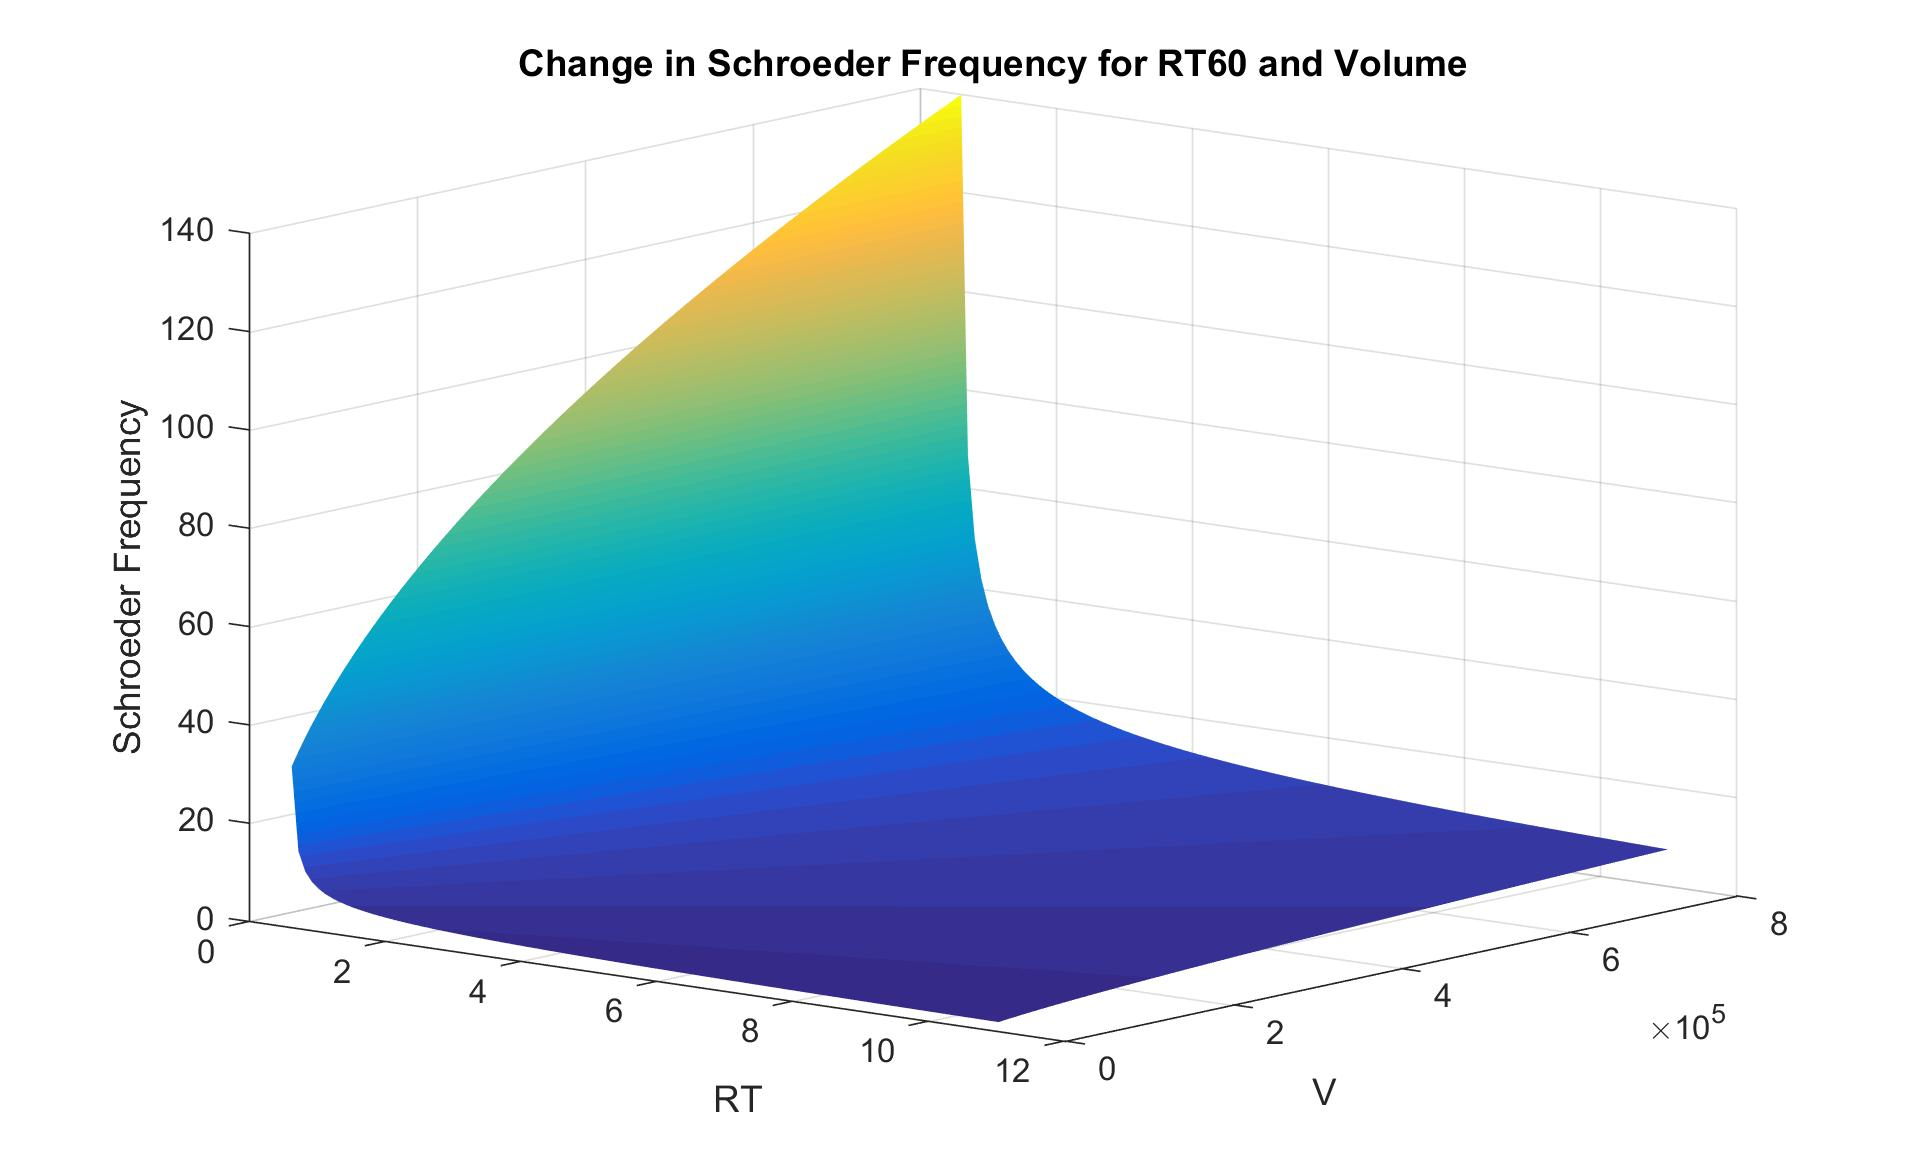
\includegraphics[width=\textwidth]{./graphics/SchroederForRTandV.jpg}
  \caption{Schroeder frequency as a function of domain size and RT60}
\end{figure}

Thus for very large domains domains with a short $RT_{60}$, modal analysis may be neither appropriate or necessary.